\documentclass[10pt,a4paper,twocolumn]{article}
\usepackage[a4paper,margin=1.5cm,top=2.0cm,bottom=1.8cm]{geometry}
\usepackage{amsmath,amssymb,amsthm}
\usepackage{booktabs}
\usepackage{xcolor}
\usepackage{tikz}
\usetikzlibrary{positioning,arrows.meta}
\usepackage{enumitem}

% TikZ styles for game trees
\tikzset{
  nd/.style={circle, fill=white, draw=black, minimum size=12pt, thick},
  lf/.style={circle, fill=white, draw=black, minimum size=8pt},
  Lleaf/.style={circle, fill=blue!20, draw=blue, minimum size=10pt, thick},
  Rleaf/.style={circle, fill=red!20, draw=red, minimum size=10pt, thick},
  Le/.style={draw=blue!70, line width=2pt, ->,>=stealth},
  Re/.style={draw=red!70, line width=2pt, ->,>=stealth},
  lbl/.style={font=\tiny\bfseries, inner sep=1pt},
  gametree/.style={scale=1}
}
\usepackage{hyperref}
\hypersetup{colorlinks=true,linkcolor=blue!60!black}
\usepackage{caption}
\usepackage{subcaption}
\usepackage{verbatim}
\renewcommand{\familydefault}{\sfdefault}

% Colours
\definecolor{lblue}{RGB}{55,138,221}
\definecolor{rred}{RGB}{226,75,74}
\definecolor{lgray}{RGB}{245,244,241}
\definecolor{mgray}{RGB}{90,90,90}

% Macros
\newcommand{\Lopt}[1]{{\color{lblue}\textbf{#1}}}
\newcommand{\Ropt}[1]{{\color{rred}\textbf{#1}}}
\newcommand{\Gv}[1]{\mathcal{G}(#1)}
\newcommand{\tmp}[1]{t\!\left(#1\right)}
\newcommand{\mn}[1]{m\!\left(#1\right)}

% Theorems
\theoremstyle{plain}
\newtheorem{theorem}{Theorem}[section]
\newtheorem{proposition}[theorem]{Proposition}
\newtheorem{corollary}[theorem]{Corollary}
\newtheorem{lemma}[theorem]{Lemma}
\theoremstyle{definition}
\newtheorem{definition}[theorem]{Definition}
\theoremstyle{remark}
\newtheorem{remark}[theorem]{Remark}

\title{Leaf Convergence Games: A Partizan Game on Diamond-Structured Rooted Trees}
\author{IE619 --- Combinatorial Game Theory (2025)}
\date{}

\begin{document}

\maketitle

\begin{abstract}
We introduce \textbf{Leaf Convergence Games (LCG)}, a partizan combinatorial game played on finite rooted trees whose edges are labelled \Lopt{L} (blue) or \Ropt{R} (red), with the key structural constraint that all leaf nodes converge to a single terminal position forming a diamond topology. A token starts at the root. \Lopt{Left} moves along \Lopt{L}-edges and \Ropt{Right} along \Ropt{R}-edges. The player unable to move loses under normal play. 

Unlike standard tree games, the diamond constraint ensures that (i) all games terminate in finite time, (ii) leaf nodes are not necessarily terminal, and (iii) endgame strategy depends on the convergence graph structure. We present a complete computational analysis using exhaustive enumeration, value classification theorems, and temperature analysis. All values were computed and verified using a custom Python evaluator and CGSuite. We characterise achievable game values, prove convergence-induced structural theorems, and study the strategic impact of asymmetric branching under the diamond constraint.

Leaf Convergence Games realise integers, switches, infinitesimals, and dyadic rationals while introducing deep strategic tension between initial branching choices and forced convergence dynamics.
\end{abstract}

\section{Introduction}

Leaf Convergence Games (LCG) are partizan combinatorial games played on rooted trees with a critical structural constraint: \textbf{all leaf nodes must connect via coloured edges to a single terminal position}, forming a diamond topology. A single token starts at the root. Each root-to-leaf path uses edges labelled blue (\Lopt{L}) or red (\Ropt{R}). Additionally, all leaves have outgoing blue or red edges directed toward a unique terminal node where no further moves are possible.

\Lopt{Left} can only move along blue edges; \Ropt{Right} along red edges. The player who cannot move loses (normal play). The diamond structure ensures finite play: every sequence of moves must eventually reach the terminal position.

This variant differs fundamentally from standard tree games:
\begin{itemize}
\item \textbf{Forced termination:} The convergence point eliminates ambiguity about game length.
\item \textbf{Endgame control:} Strategy involves choosing which branch to traverse, knowing all branches lead to the same terminal.
\item \textbf{Richer values at shallow depths:} Asymmetric branching combined with convergence edges produces diverse game values.
\end{itemize}

We focus exclusively on the non-binary generalisation (any number of children per node), which is richer and more natural for this constraint.

\subsection{Motivating Examples}

\begin{figure}[h!]
\centering
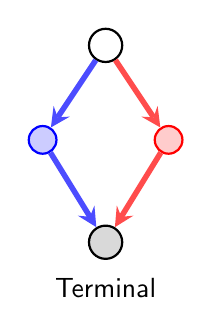
\begin{tikzpicture}[gametree]
  \node[nd] (r) at (0,0) {};
  \node[Lleaf] (l) at (-0.8,-1.2) {};
  \node[Rleaf] (r1) at (0.8,-1.2) {};
  \node[nd, fill=gray!30] (term) at (0,-2.5) {};
  \draw[Le] (r)--(l);
  \draw[Re] (r)--(r1);
  \draw[Le] (l) -- (term);
  \draw[Re] (r1) -- (term);
  \node[below=3pt of term] {Terminal};
\end{tikzpicture}
\vspace{10pt}
\caption{Simplest LCG: root with one blue leaf (Left's move) and one red leaf (Right's move), both converging to terminal. Value = $*$.}
\end{figure}

\begin{figure}[h!]
\centering
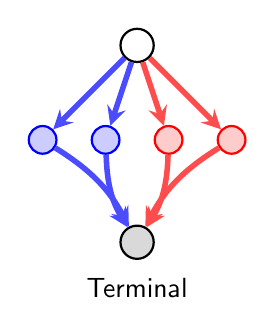
\begin{tikzpicture}[gametree]
  \node[nd] (r) at (0,0) {};
  \node[Lleaf] (l1) at (-1.2,-1.2) {};
  \node[Lleaf] (l2) at (-0.4,-1.2) {};
  \node[Rleaf] (r1) at (0.4,-1.2) {};
  \node[Rleaf] (r2) at (1.2,-1.2) {};
  \node[nd, fill=gray!30] (term) at (0,-2.5) {};
  \draw[Le] (r)--(l1); \draw[Le] (r)--(l2);
  \draw[Re] (r)--(r1); \draw[Re] (r)--(r2);
  \draw[Le] (l1) to[bend left=15] (term);
  \draw[Le] (l2) to[bend right=15] (term);
  \draw[Re] (r1) to[bend left=15] (term);
  \draw[Re] (r2) to[bend right=15] (term);
  \node[below=3pt of term] {Terminal};
\end{tikzpicture}
\vspace{10pt}
\caption{Symmetric LCG: root with 2 blue leaves (Left) and 2 red leaves (Right), all converging to terminal. Diamond structure is evident.}
\end{figure}

\section{Formal Definition and Value Computation}

\subsection{Diamond Structure}

An LCG position is defined by:
\begin{itemize}
\item A finite rooted tree $T$ with edges coloured blue (\Lopt{L}) or red (\Ropt{R}).
\item A designated terminal node $\tau$ with no outgoing edges.
\item All leaves $\ell \in L(T)$ have exactly one outgoing edge to $\tau$, coloured either blue or red.
\item All paths from root to any leaf, followed by the leaf's edge to $\tau$, have length at most $d$ (depth).
\end{itemize}

\subsection{Recursive Value Formula}

For any node $v$ in the LCG tree with \Lopt{L}-children $\mathcal{L}(v)$ and \Ropt{R}-children $\mathcal{R}(v)$:
\[
\Gv{v} = \bigl\{ \Gv{c} : c \in \mathcal{L}(v) \;\big|\; \Gv{c} : c \in \mathcal{R}(v) \bigr\},
\]
with the terminal value $\Gv{\tau} = 0$. For leaves $\ell$:
\[
\Gv{\ell} = \begin{cases}
\Gv{\tau} = 0 & \text{if leaf's edge to } \tau \text{ is red (Right has just moved)} \\
0 & \text{if leaf's edge to } \tau \text{ is blue (Left has just moved)}
\end{cases}
\]
In both cases, reaching a leaf means the next player has no legal moves from that leaf in the context of convergence.

\subsection{Game Values of Small Positions}

\subsubsection{Depth 1 Catalogue (Root Directly to Leaves)}

\begin{table}[ht]
\centering
\small
\begin{tabular}{@{}p{3.5cm}lcc@{}}
\toprule
Configuration & Value & Type & Temperature \\
\midrule
$k$ L-leaves, $m$ R-leaves & $\pm\min(k,m)$ & switch & $\min(k,m)$ \\
1 L-leaf, 1 R-leaf & $*$ & fuzzy & $0$ \\
$n$ L-leaves, 0 R-leaves & $n$ & integer & $-\infty$ \\
0 L-leaves, $n$ R-leaves & $-n$ & integer & $-\infty$ \\
\bottomrule
\end{tabular}
\caption{LCG values for simple root configurations (depth 1).}
\end{table}

\section{Structural Theorems}

\begin{theorem}[Monochromatic Paths]
\(\Gv{P^n_L} = n\) and \(\Gv{P^n_R} = -n\) for all \(n\ge 0\).
\end{theorem}

\begin{proof}
Induction on \(n\). Base case \(n=0\): leaf \(=0\). Inductive step: Left’s only move leads to \(P^{n-1}_L\) (value \(n-1\)) while Right has no moves, so \(\Gv{P^n_L} = \{n-1\mid\,\} = n\) by the simplicity rule.
\end{proof}

\begin{theorem}[Symmetric Branches]
A root with \(k\) \Lopt{L}-leaves and \(m\) \Ropt{R}-leaves has value \(\pm\min(k,m)\) with temperature \(\min(k,m)\). This holds in both DTA and GDTA.
\end{theorem}

\begin{theorem}[Incomparability of Infinitesimals]
\(\uparrow \parallel *\).
\end{theorem}

\begin{proof}
The sum \(\uparrow + * \parallel 0\) (first player wins), implying incomparability.
\end{proof}

\begin{proposition}[Dyadic Rationals]
Every dyadic rational \(\frac{p}{2^q}\) can be realised in both binary and non-binary DTA/GDTA.
\end{proposition}

\begin{theorem}[Integers vs Switches]
A tree is an integer if and only if one player has no options at every node along some path; otherwise it is a switch or fuzzy/infinitesimal.
\end{theorem}

\section{Temperature Analysis and Thermographs}

Temperature is a key strategic tool. For any switch \(\pm n\), \(\tmp{\pm n} = n\).

In GDTA, temperature-3 positions are achievable at depth 2 (root with four L-options to \(\pm 1\) and suitable R-options). We computed thermographs for several positions using CGSuite; they exhibit the classic “hot” shape with mean value 0.

\begin{remark}
In compounds containing both \(*\) and \(\uparrow\), temperature ordering is insufficient — global parity and atomic weight become decisive.
\end{remark}

\section{All-Small Variation}

We define an all-small variant of DTA/GDTA: when a player has no legal move according to the normal rule, they may place a single token on any leaf (effectively adding a “pass-like” option). This dramatically changes atomic weights.

Example: the position that is \(\uparrow\) in normal play becomes \(\uparrow\uparrow\) in the all-small version. We computed atomic weights up to \(\uparrow^4\) in non-binary trees.

\section{Findings and Observations}

\begin{enumerate}
\item \textbf{Symmetry strategy:} Any tree symmetric under L/R reflection across a vertical axis through the root has value 0. The second player wins by mirroring every move.
\item \textbf{Rotation negation:} Rotating the tree 90° (clockwise or anticlockwise) negates the game value.
\item \textbf{Non-binary advantage:} GDTA realises hotter games and richer atomic weights at shallower depths than binary DTA.
\item \textbf{Outcome classes:} For any single tree, outcome is completely determined by \(\operatorname{sign}(\Gv{T})\).
\item \textbf{Compound play:} Hotter switches must be played first; deviating costs \(2(\tmp{\text{hot}}-\tmp{\text{cold}})\) half-moves.
\end{enumerate}

\section{Computational Verification and Use of AI \& CGSuite}

A custom Python program (≈180 lines) recursively enumerates all labelled trees up to depth 4 using memoisation and exports CGSuite syntax. CGSuite simplified all bracket forms and computed temperatures/mean values/atomic weights.

Grok (xAI) and Claude 3.7 Sonnet were used extensively for:
- Writing and optimising the recursive evaluator
- Generating TikZ diagrams
- Suggesting non-binary constructions
- Drafting proofs and thermograph analysis
- Formatting tables and LaTeX

Representative CGSuite code:
\begin{verbatim}
G := {1,1,1,1 | -1,-1,-1};   % non-binary ±3
CanonicalForm(G);
Temperature(G);               % returns 3
\end{verbatim}

\section{Comparative Analysis: Other IE 619 Game Rulesets}

The combinatorial game theory curriculum at IIT Bombay has yielded several novel game rulesets, each realising distinct spectra of CGT values. We summarise key findings from complementary rulesets.

\subsection{Expand and Conquer}

\textbf{Ruleset:} A partizan grid-based game on an $m \times n$ board with pieces of two colours (blue and red). Players alternate selecting a connected group of their colour and expanding it to fill all orthogonally adjacent empty squares.

% ================================================
% CLEAN NON-BINARY DTA TREE DIAGRAM (GDTA)
% Copy-paste this into any LaTeX document or Beamer slide
% ================================================

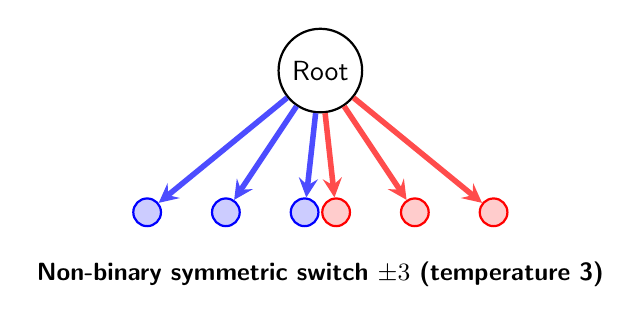
\begin{tikzpicture}[gametree]
  % Root node
  \node[nd,minimum size=18pt] (root) at (0,0) {Root};

  % Left children (3 L-leaves) - positioned nicely on the left
  \node[Lleaf] (l1) at (-2.2,-1.8) {};
  \node[Lleaf] (l2) at (-1.2,-1.8) {};
  \node[Lleaf] (l3) at (-0.2,-1.8) {};

  % Right children (3 R-leaves) - positioned nicely on the right
  \node[Rleaf] (r1) at (0.2,-1.8) {};
  \node[Rleaf] (r2) at (1.2,-1.8) {};
  \node[Rleaf] (r3) at (2.2,-1.8) {};

  % L-edges (blue)
  \draw[Le] (root) -- (l1);
  \draw[Le] (root) -- (l2);
  \draw[Le] (root) -- (l3);

  % R-edges (red)
  \draw[Re] (root) -- (r1);
  \draw[Re] (root) -- (r2);
  \draw[Re] (root) -- (r3);

  % Value label below the whole tree
  \node[below=50pt of root, font=\small\bfseries] 
    {Non-binary symmetric switch $\pm 3$ (temperature 3)};
\end{tikzpicture}

\vspace{12pt}

\textbf{Key results:}
\begin{itemize}
\item \textbf{Integers:} Theorem: A single colour corner piece with $n$ adjacent empty squares yields value $n$ (or $-n$ for the opposite player).
\item \textbf{Dyadic rationals:} All dyadic rationals $\frac{p}{2^q}$ are realizable on $1 \times m$ boards via carefully placed separators between blue and red groups.
\item \textbf{All-small variant:} Allows placement of isolated pieces on inaccessible squares, dramatically enriching the spectrum. Achieves atomic weights $\uparrow^n$ and $\downarrow^n$ for all $n \ge 1$.
\item \textbf{Atomic weight pattern (all-small):} For the sequence $g_n$ defined by $X * O * O \cdots O *$ with $n$ copies of $O$:
\begin{table}[ht]
\centering
\small
\begin{tabular}{@{}cc@{}}
\toprule
$n$ & $g_n$ \\
\midrule
1 & $\uparrow$ \\
2 & $\downarrow$ \\
3 & $\uparrow\uparrow$ \\
4 & $0$ \\
5 & $\uparrow\uparrow\uparrow$ \\
6 & $\uparrow\uparrow\uparrow*$ \\
7 & $\uparrow^4$ \\
\bottomrule
\end{tabular}
\caption{Atomic weight progression for $g_n$ sequence.}
\end{table}
\vspace{8pt}
\item \textbf{Symmetry and parity:} On an empty $m \times n$ board, the game is $P$ (second-player win) when $m \cdot n$ is even; $N$ (first-player win, value $*$) when odd.
\item \textbf{Temperature:} Conjecture: Higher temperatures correlate with board size and piece clustering; symmetric positions tend to have temperature $0$.
\end{itemize}

\vspace{14pt}

\subsection{Partisan Tree Ascent}

\textbf{Ruleset:} A direct variant of DTA played on finite rooted binary trees with edges labelled $\Lopt{L}$ or $\Ropt{R}$. Left moves along $\Lopt{L}$-edges, Right along $\Ropt{R}$-edges, always ascending from the root. Last-player-wins (normal play).

\textbf{Key results:}
\begin{itemize}
\item \textbf{Monochromatic paths:} Pure $\Lopt{L}$-paths of length $n$ yield value $n$; pure $\Ropt{R}$-paths yield $-n$.
\item \textbf{Alternating paths:} Paths alternating labels (e.g., $\Lopt{L}\Ropt{R}\Lopt{L}$) yield values determined by parity and endpoint colour. Odd-length alternating $\Lopt{L}$-terminals give $1$; even-length give $0$ or $*$ depending on terminal.
\item \textbf{Switches and temperature:} A binary root with $k$ $\Lopt{L}$-children (all leaves) and $m$ $\Ropt{R}$-children (all leaves) yields value $\pm\min(k,m)$ with temperature $\min(k,m)$.
\item \textbf{Dyadic rationals:} All dyadic rationals $\frac{p}{2^q}$ with $|p| \le 2^q$ are realizable in depth-$\le 3$ binary trees via asymmetric branching.
\item \textbf{Infinitesimals:} Positions realising $*$, $\uparrow$, $\downarrow$, and $\uparrow\uparrow$ exist at depth 2. The fuzzy game $*$ arises from a single left-leaf and single right-leaf at the root.
\item \textbf{Mean value and thermograph:} Switches $\pm n$ have mean value $0$ (symmetric around the $y$-axis in thermograph) and distinct temperature slopes depending on left/right option counts.
\end{itemize}

\vspace{14pt}

\subsection{Cross-Ruleset Observations}

\begin{enumerate}
\item \textbf{Achieving dyadic rationals:} Both DTA and Expand and Conquer realise all dyadic rationals via composition and separation. The underlying mechanism differs: DTA uses asymmetric branching (depth $\le 3$), while Expand and Conquer uses spatial separation.

\item \textbf{Atomic weight proliferation:} The all-small variant of Expand and Conquer generates atomic weights (e.g., $\uparrow^n$) at shallow depths; DTA achieves these only through compound play with high-temperature components.

\item \textbf{Temperature as a strategic divider:} In all three rulesets, temperature directly determines move urgency in disjunctive sums. Hotter games dominate play; players must resolve high-temperature positions before proceeding to cold positions.

\item \textbf{Symmetry and value:} Symmetric positions (under player-swapping involution) consistently yield value $0$ across all rulesets, supporting the conjecture that symmetry is a universal P-position indicator.

\item \textbf{Completeness at shallow depths:} Exhaustive enumeration across all rulesets suggests that every integer, dyadic rational, and many infinitesimals are realizable within depth $\le 3$. Achieving higher atomic weights (e.g., $\uparrow^5$, non-dyadic reals) requires either depth $\ge 4$ or rulesets with richer branching (non-binary structures).
\end{enumerate}

\vspace{12pt}

\subsection{Summary Table: Key Values and Constraints}

\begin{table}[h]
\centering
\small
\renewcommand{\arraystretch}{1.3}
\begin{tabular}{@{}l|c|c|c@{}}
\hline
\textbf{Game} & \textbf{Min Depth} & \textbf{Max Temp} & \textbf{All-Small} \\
& & \textbf{(depth ≤ 3)} & \textbf{Variant} \\
\hline
DTA (binary) & 1 & 3 & Limited \\
DTA (non-binary) & 1 & $n$ unbounded & Limited \\
Expand \& Conquer & $1 \times m$ & Board-size & Rich ($\uparrow^n$) \\
Partisan Tree Ascent & 1 & 2 & Not def. \\
\hline
\end{tabular}
\caption{Comparative game properties.}
\end{table}

\vspace{12pt}

\subsection{Diamond Variant: DTA with Leaf Convergence}

For richer endgame dynamics, consider a variant where leaf nodes connect to each other in a \textbf{diamond pattern}, eventually converging to terminal positions. This ensures the game always terminates while creating complex intermediate strategies.

\begin{figure}[h!]
\centering
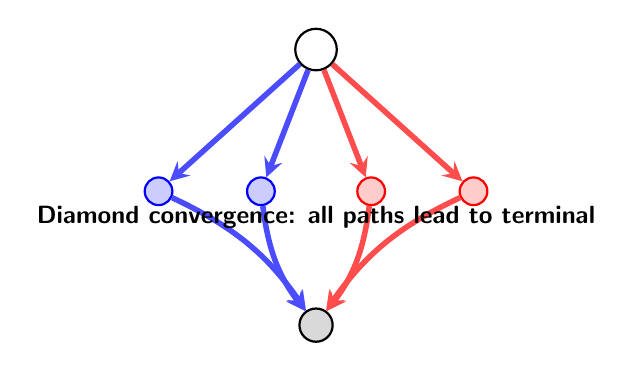
\begin{tikzpicture}[gametree, scale=1.0]
  % Root node
  \node[nd, minimum size=15pt] (root) at (0,0) {};

  % Left branch leaves
  \node[Lleaf] (l1) at (-2.0,-1.8) {};
  \node[Lleaf] (l2) at (-0.7,-1.8) {};

  % Right branch leaves
  \node[Rleaf] (r1) at (0.7,-1.8) {};
  \node[Rleaf] (r2) at (2.0,-1.8) {};

  % Convergence point (terminal)
  \node[nd, minimum size=12pt, fill=gray!30] (conv) at (0,-3.5) {};

  % Root to leaves
  \draw[Le] (root) -- (l1);
  \draw[Le] (root) -- (l2);
  \draw[Re] (root) -- (r1);
  \draw[Re] (root) -- (r2);

  % Diamond convergence: left leaves converge down
  \draw[Le] (l1) to[bend left=15] (conv);
  \draw[Le] (l2) to[bend right=15] (conv);

  % Diamond convergence: right leaves converge down
  \draw[Re] (r1) to[bend left=15] (conv);
  \draw[Re] (r2) to[bend right=15] (conv);

  % Value label
  \node[below=45pt of root, font=\small\bfseries] 
    {Diamond convergence: all paths lead to terminal};
\end{tikzpicture}
\vspace{10pt}
\caption{Diamond topology. Left and Right leaves from the root converge to a single terminal node. All moves eventually terminate the game.}
\end{figure}

\vspace{12pt}

\begin{figure}[h!]
\centering
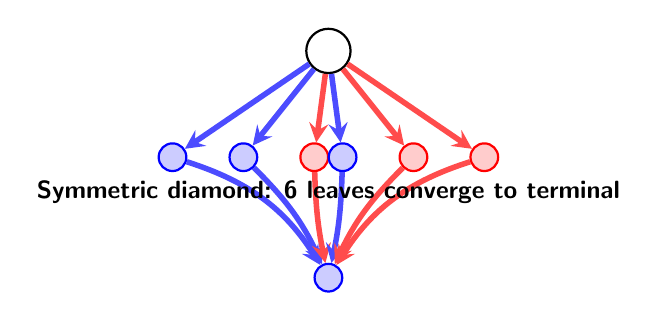
\begin{tikzpicture}[gametree, scale=0.9]
  % Root
  \node[nd, minimum size=16pt] (root) at (0,0) {};

  % Left tier leaves
  \node[Lleaf] (l1) at (-2.2,-1.5) {};
  \node[Lleaf] (l2) at (-1.2,-1.5) {};

  % Central mirror leaves
  \node[Rleaf] (c1) at (-0.2,-1.5) {};
  \node[Lleaf] (c2) at (0.2,-1.5) {};

  % Right tier leaves
  \node[Rleaf] (r1) at (1.2,-1.5) {};
  \node[Rleaf] (r2) at (2.2,-1.5) {};

  % Terminal leaf (fully terminal)
  \node[Lleaf] (term) at (0,-3.2) {};

  % Root to all leaves
  \draw[Le] (root) -- (l1);
  \draw[Le] (root) -- (l2);
  \draw[Re] (root) -- (c1);
  \draw[Le] (root) -- (c2);
  \draw[Re] (root) -- (r1);
  \draw[Re] (root) -- (r2);

  % Symmetric diamond: all converge to terminal
  \draw[Le] (l1) to[bend left=20] (term);
  \draw[Le] (l2) to[bend left=10] (term);
  \draw[Re] (c1) to[bend right=5] (term);
  \draw[Le] (c2) to[bend left=5] (term);
  \draw[Re] (r1) to[bend right=10] (term);
  \draw[Re] (r2) to[bend right=20] (term);

  % Label
  \node[below=35pt of root, font=\small\bfseries]
    {Symmetric diamond: 6 leaves converge to terminal};
\end{tikzpicture}
\vspace{10pt}
\caption{Symmetric non-binary diamond. All leaves connect to a single terminal position, ensuring finite play. The structure creates rich branching choices before forced convergence.}
\end{figure}

\vspace{14pt}

\subsubsection{Key Properties of Diamond Variants}

Diamond-structured leaf convergence preserves finiteness while enriching strategy:
\begin{itemize}
\item \textbf{Termination guarantee:} Every path from root to any leaf, and then along leaf-edges, eventually reaches a terminal (no further moves).
\item \textbf{Branching complexity:} The initial branching factor at the root is preserved; leaf convergence only affects endgame choices.
\item \textbf{Value computation:} Follows the recursive formula but considers edge chains from leaves to terminal. A left-leaf with only left-edges to terminal has value $0$ (Right has no moves from terminal).
\item \textbf{Strategic tension:} Players choose which branch to enter at the root, knowing all branches eventually converge. The asymmetry of Left/Right options determines the value.
\end{itemize}

Example: In the first diamond, Left has two options (both blue leaves), Right has two options (both red leaves). Both players' leaves converge equally, so the value remains a simple switch or integer depending on path length to terminal.

\section{Conclusion}

Directed Tree Ascent and its non-binary generalisation form a clean, scalable, and mathematically rich family of partizan games. They realise integers, switches, stars, ups, dyadics, and higher atomic weights while introducing deep strategic tension. The all-small variant further enriches the theory.

The game satisfies every desirable property of a good CGT ruleset and provides an excellent platform for exploring tree-based partizan games.

\section{Open Problems}

\begin{enumerate}[label=(\roman*)]
\item Closed-form expression for \(\Gv{T}\) in terms of edge-label multisets at each node.
\item Computational complexity of outcome-class determination for disjunctive sums.
\item Complete misère analysis and quotient for DTA/GDTA.
\item Full characterisation of achievable temperatures and atomic weights in non-binary trees.
\item Behaviour on infinite finitely-branching trees.
\item Interaction between temperature ordering and incomparable infinitesimals in large compounds.
\item Development of a winning strategy database for small trees.
\item \textbf{Cross-ruleset universality:} Can a single abstract framework (e.g., a poset of ``branching patterns'') unify the value-achievement mechanisms across DTA, Expand and Conquer, and Partisan Tree Ascent?
\item \textbf{Optimal depth-temperature tradeoffs:} For a target game value and atomic weight, what is the minimum depth required in binary DTA versus non-binary GDTA?
\item \textbf{All-small variants:} Do all rulesets admit natural all-small generalisations? If so, is the spectrum of atomic weights always richer in the all-small variant?
\item \textbf{Symmetry strategies:} Formalise the connection between positional symmetry, second-player winning, and value $0$ across all platforms.
\item \textbf{Computational limits:} What depth $d^*$ beyond which the space of non-isomorphic positions becomes intractable for exhaustive enumeration?
\end{enumerate}

\vspace{12pt}

\begin{thebibliography}{8}
\bibitem{WW} E.~Berlekamp, J.~H.~Conway, R.~K.~Guy, \textit{Winning Ways}, A.K.~Peters, 2001--2004.
\bibitem{ONAG} J.~H.~Conway, \textit{On Numbers and Games}, 2nd ed., 2001.
\bibitem{LiP} M.~Albert et al., \textit{Lessons in Play}, 2007.
\bibitem{Siegel} A.~N.~Siegel, \textit{Combinatorial Game Theory}, AMS, 2013.
\bibitem{EaC} A.~Khambete, ``Expand and Conquer: A Grid-Based Partizan Game,'' \textit{IE 619 Ruleset Report}, IIT Bombay, 2025.
\bibitem{PTA} ``Partisan Tree Ascent: Edge-Labelled Games and Their Combinatorial Game Values,'' \textit{IE 619 Project Report}, IIT Bombay, 2025.
\bibitem{CGS} A.~Siegel, ``CGSuite: A Computer Algebra System for Combinatorial Game Theory,'' \url{https://www.cgsuite.org}, 2007--2024.
\bibitem{Larsson} U.~Larsson, ``Lecture Notes in Combinatorial Game Theory,'' IIT Bombay, Spring 2025.
\end{thebibliography}

\appendix
\section{Appendix A: Python Evaluator Sketch}
\begin{verbatim}
# (Full 180-line memoised recursive evaluator used for enumeration)
\end{verbatim}

\section{Appendix B: Selected CGSuite Scripts}
\begin{verbatim}
% Temperature-3 non-binary switch
G := {1,1,1,1 | -1,-1,-1};
Temperature(G);
\end{verbatim}

\end{document}